\documentclass{article}
\usepackage{amsmath, fullpage}
\usepackage{graphicx}
\usepackage[portuguese]{babel}
\usepackage{fancyhdr}
\usepackage{lastpage}

\graphicspath{{figures/}}

\pagestyle{fancy}
\fancyhf{} % limpa tudo

\fancyhead[L]{
\includegraphics[height=1.2cm]{Logo_UnB.png}}
\fancyhead[R]{
\includegraphics[height=1.2cm]{Logo_Vertical_01.png}}

\renewcommand{\headrulewidth}{0.4pt} % linha do cabeçalho (opcional)

\setlength{\headheight}{1.5cm}
\setlength{\headsep}{0.8cm}

\begin{document}

\title{Manual de operação: ComMarker B6 MOPA Fiber Laser Engraver}
\author{Henrique de O. Bernardes}
%\date{\vspace{-5ex}}
\maketitle
\thispagestyle{fancy} % garante cabeçalho na primeira página

\section{Identificação do Documento}
\textbf{Equipamento: ComMarker B6 MOPA Fiber Laser Engraver}\\
\textbf{Categoria: Gravadora}\\

\subsection{Controle de Revisões}
\begin{center}
\begin{tabular}{|c|c|p{8cm}|}
\hline
\textbf{Versão} & \textbf{Data} & \textbf{Descrição} \\
\hline
1.0 & --- & Manual técnico inicial \\
\hline
% Adicione novas linhas aqui
% 1.1 & 01/01/2025 & Atualização de conteúdo \\
% \hline
\end{tabular}
\end{center}
\section{Objetivo}
O objetivo deste manual de operação é fornecer orientações para o uso adequado da \textbf{ComMarker B6 MOPA Fiber Laser Engraver}, assegurando que o operador seja capaz de operar o equipamento de forma segura, eficiente e com alto padrão de qualidade. Este documento busca ainda minimizar riscos associados à operação do laser, prevenir danos ao equipamento e aos materiais processados, além de auxiliar na identificação e solução de possíveis falhas. Adicionalmente, o manual tem como finalidade padronizar procedimentos, facilitar o treinamento de novos usuários e garantir o melhor desempenho do sistema ao longo de sua vida útil.
\section{Visão Geral Da Gravadora}
A ComMarker B6 MOPA Fiber Laser Engraver é uma gravadora a laser de fibra com potência de 60W. O equipamento utiliza tecnologia de laser do tipo MOPA (Master Oscillator Power Amplifier), operando  no comprimento de onda de 1064 nm, sendo possível realizar gravações, marcações e cortes em metais e alguns materiais não metálicos. Dentre os materiais principais que podem ser gravados de acordo com a fabricante estão:
\begin{itemize}
  \item Cobre
  \item Alumínio
  \item Acrílico
  \item Prata
  \item Aço inoxidável
  \item Plástico
\end{itemize}
\begin{figure}
  \begin{center}
    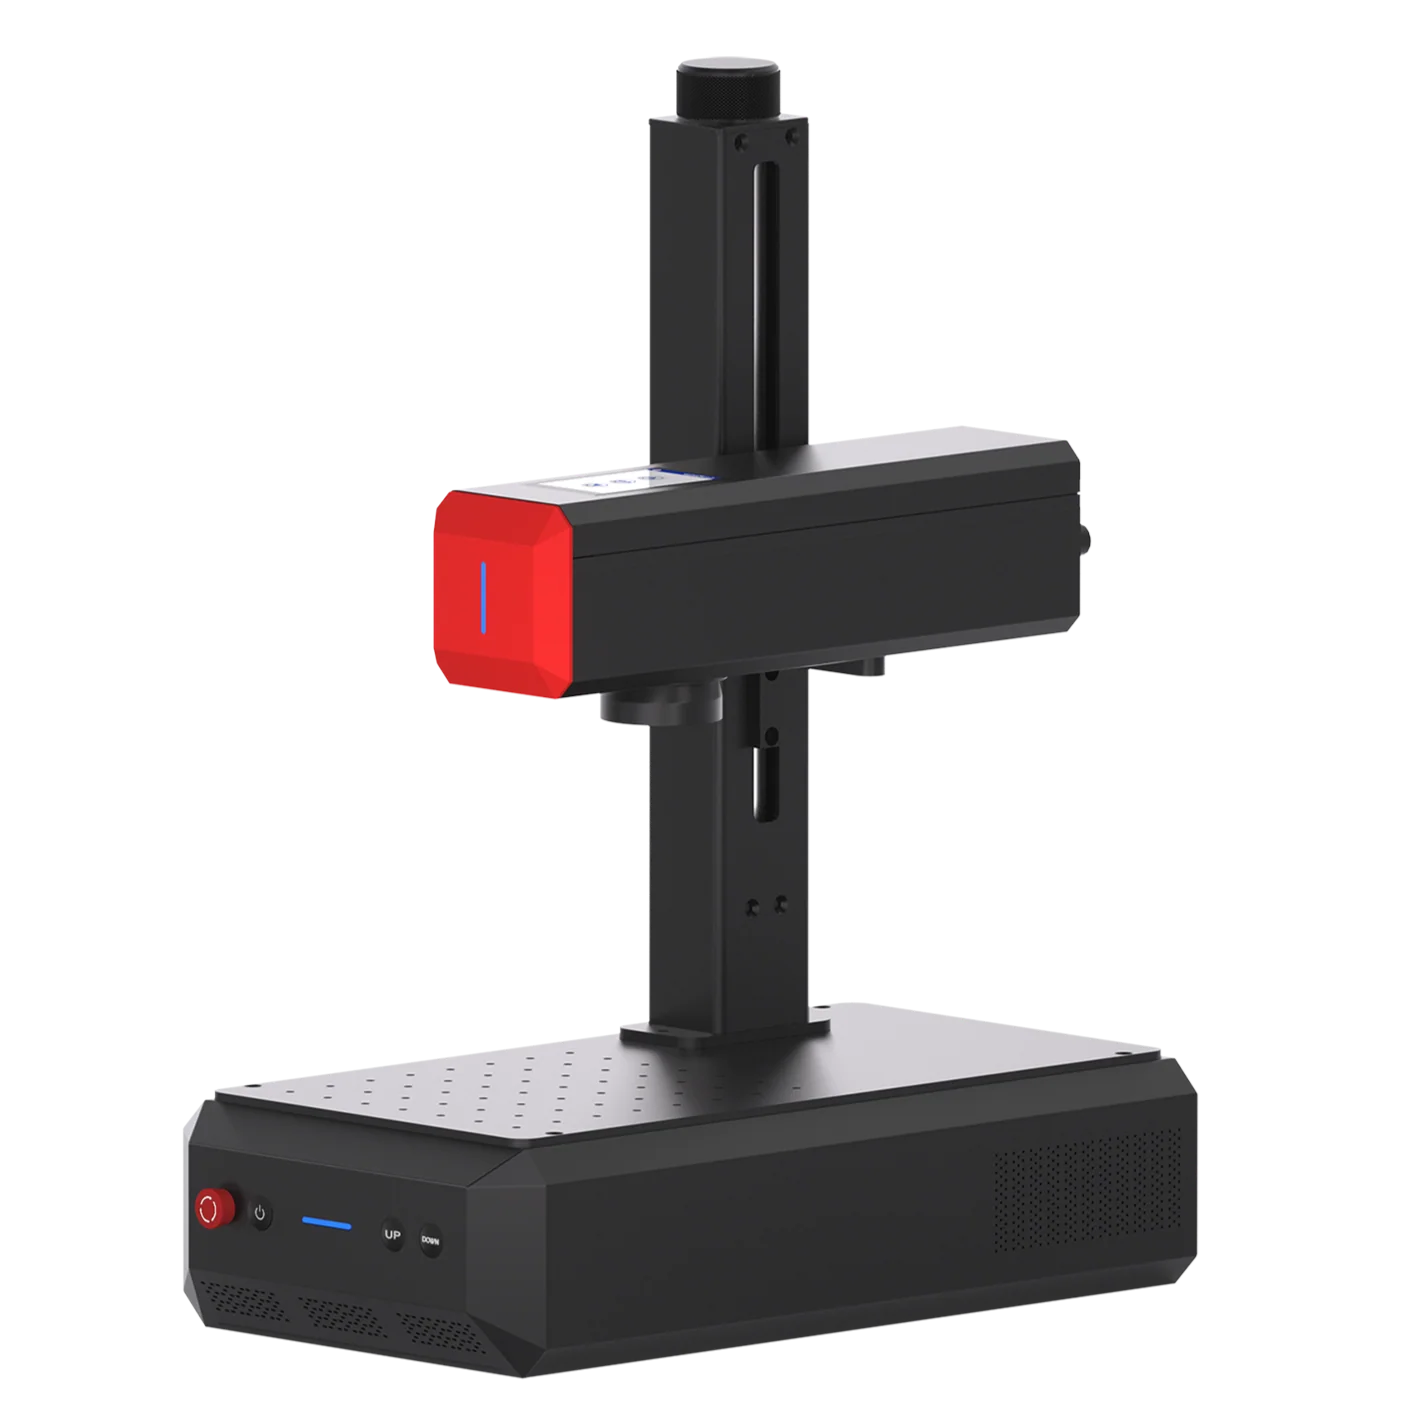
\includegraphics[width=0.45\textwidth]{figures/B6Mopa.jpg}
  \end{center}
  \caption{ComMarker B6 MOPA Fiber Laser Engraver}\label{fig:}
\end{figure}

\section{Identificação dos Componentes}
\begin{figure}[h]
  \centering
  \begin{minipage}{0.50\textwidth}
    \centering
    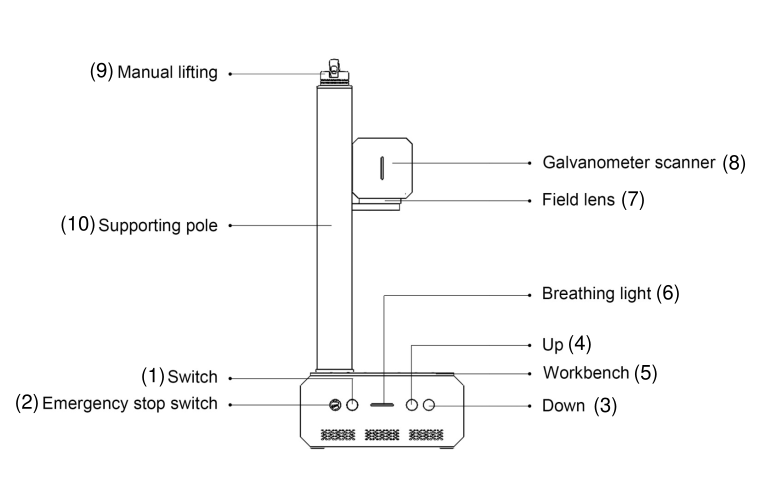
\includegraphics[width=\linewidth]{figures/frenteB6Anotada.png}
    \caption{Visão frontal da gravadora}
  \end{minipage}\hfill
  \begin{minipage}{0.50\textwidth}
    \centering
    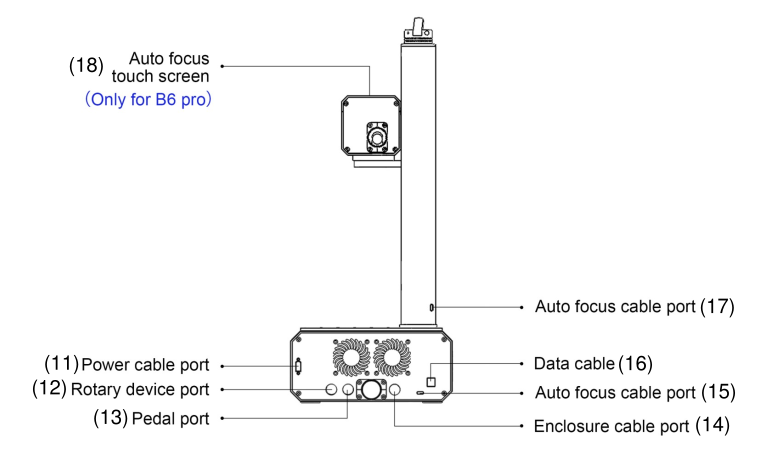
\includegraphics[width=\linewidth]{figures/trasB6Anotada.png}
    \caption{Visão traseira da gravadora}
  \end{minipage}
\end{figure}
\begin{enumerate}
  \item Switch: Botão de liga/desliga;
  \item Emergency stop switch: Chave de parada de emergência;
  \item Down: Movimentação do conjunto do laser para baixo;
  \item Up: Movimentação do conjunto do laser para cima;
  \item Workbench: Bancada/Superfície de trabalho;
  \item Breathing light: Luz indicadora de estado(ligado/desligado);
  \item Field lens: Lente de campo;
  \item Galvanometer scanner: Scanner galvanometro;
  \item Manual lifting: Elevadora manual do conjunto laser;
  \item Supporting pole: Coluna de suporte;
  \item Power cable port: Porta do cabo de alimentação;
  \item Rotary device port: Porta do eixo rotativo;
  \item Pedal port: Porta para pedal;
  \item Enclosure cable port: ?;
  \item Auto focus cable port: Porta para cabo do foco automático;
  \item Data cable: Cabo de dados(USB);
  \item Auto focus cable port: Porta para cabo do foco automático;
  \item Auto focus touch screen: Tela para foco automático.
\end{enumerate}

\section{Materiais de Gravação}
\section{Parâmetros de Impressão Recomendados}

\newpage
\section{Fluxograma Operacional do Processo}
Na imagem \ref{fig:fluxogramaOperacionalGravadora} vemos o fluxograma operacional do processo de gravação:
\begin{figure}[!h]
  \begin{center}
    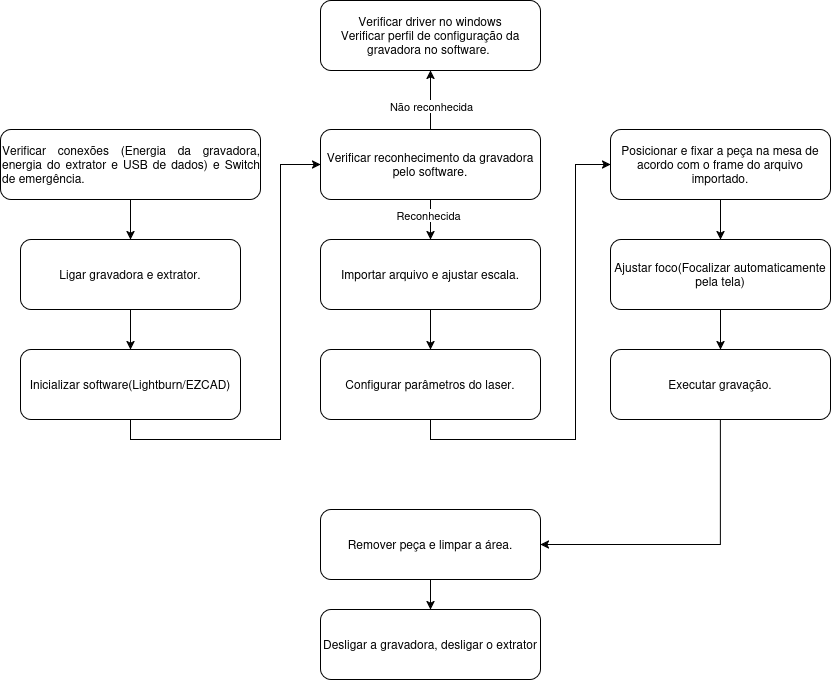
\includegraphics[width=0.75\textwidth]{figures/MOPADiagrama.png}
  \end{center}
  \caption{Fluxograma operacional da gravadora}\label{fig:fluxogramaOperacionalGravadora}
\end{figure}


\section{Procedimento Operacional}
\section{Checklist de Pré-Impressão}
\section{Preparação da Mesa}
\section{Calibração}
\section{Início da Impressão}
\section{Monitoramento}
\section{Troubleshooting}
\section{Remoção da placa}
\section{Manutenção Básica}
\section{Checklist de Pós-Impressão}
\section{Critérios de Qualidade da Impressão}
\section{Referências}
\newpage
\end{document}
